% Options for packages loaded elsewhere
\PassOptionsToPackage{unicode}{hyperref}
\PassOptionsToPackage{hyphens}{url}
%
\documentclass[
]{ctexart}
\usepackage{amsmath,amssymb}
\usepackage{iftex}
\ifPDFTeX
  \usepackage[T1]{fontenc}
  \usepackage[utf8]{inputenc}
  \usepackage{textcomp} % provide euro and other symbols
\else % if luatex or xetex
  \usepackage{unicode-math} % this also loads fontspec
  \defaultfontfeatures{Scale=MatchLowercase}
  \defaultfontfeatures[\rmfamily]{Ligatures=TeX,Scale=1}
\fi
\usepackage{lmodern}
\ifPDFTeX\else
  % xetex/luatex font selection
\fi
% Use upquote if available, for straight quotes in verbatim environments
\IfFileExists{upquote.sty}{\usepackage{upquote}}{}
\IfFileExists{microtype.sty}{% use microtype if available
  \usepackage[]{microtype}
  \UseMicrotypeSet[protrusion]{basicmath} % disable protrusion for tt fonts
}{}
\makeatletter
\@ifundefined{KOMAClassName}{% if non-KOMA class
  \IfFileExists{parskip.sty}{%
    \usepackage{parskip}
  }{% else
    \setlength{\parindent}{0pt}
    \setlength{\parskip}{6pt plus 2pt minus 1pt}}
}{% if KOMA class
  \KOMAoptions{parskip=half}}
\makeatother
\usepackage{xcolor}
\usepackage[margin=2cm]{geometry}
\usepackage{color}
\usepackage{fancyvrb}
\newcommand{\VerbBar}{|}
\newcommand{\VERB}{\Verb[commandchars=\\\{\}]}
\DefineVerbatimEnvironment{Highlighting}{Verbatim}{commandchars=\\\{\}}
% Add ',fontsize=\small' for more characters per line
\usepackage{framed}
\definecolor{shadecolor}{RGB}{248,248,248}
\newenvironment{Shaded}{\begin{snugshade}}{\end{snugshade}}
\newcommand{\AlertTok}[1]{\textcolor[rgb]{0.94,0.16,0.16}{#1}}
\newcommand{\AnnotationTok}[1]{\textcolor[rgb]{0.56,0.35,0.01}{\textbf{\textit{#1}}}}
\newcommand{\AttributeTok}[1]{\textcolor[rgb]{0.13,0.29,0.53}{#1}}
\newcommand{\BaseNTok}[1]{\textcolor[rgb]{0.00,0.00,0.81}{#1}}
\newcommand{\BuiltInTok}[1]{#1}
\newcommand{\CharTok}[1]{\textcolor[rgb]{0.31,0.60,0.02}{#1}}
\newcommand{\CommentTok}[1]{\textcolor[rgb]{0.56,0.35,0.01}{\textit{#1}}}
\newcommand{\CommentVarTok}[1]{\textcolor[rgb]{0.56,0.35,0.01}{\textbf{\textit{#1}}}}
\newcommand{\ConstantTok}[1]{\textcolor[rgb]{0.56,0.35,0.01}{#1}}
\newcommand{\ControlFlowTok}[1]{\textcolor[rgb]{0.13,0.29,0.53}{\textbf{#1}}}
\newcommand{\DataTypeTok}[1]{\textcolor[rgb]{0.13,0.29,0.53}{#1}}
\newcommand{\DecValTok}[1]{\textcolor[rgb]{0.00,0.00,0.81}{#1}}
\newcommand{\DocumentationTok}[1]{\textcolor[rgb]{0.56,0.35,0.01}{\textbf{\textit{#1}}}}
\newcommand{\ErrorTok}[1]{\textcolor[rgb]{0.64,0.00,0.00}{\textbf{#1}}}
\newcommand{\ExtensionTok}[1]{#1}
\newcommand{\FloatTok}[1]{\textcolor[rgb]{0.00,0.00,0.81}{#1}}
\newcommand{\FunctionTok}[1]{\textcolor[rgb]{0.13,0.29,0.53}{\textbf{#1}}}
\newcommand{\ImportTok}[1]{#1}
\newcommand{\InformationTok}[1]{\textcolor[rgb]{0.56,0.35,0.01}{\textbf{\textit{#1}}}}
\newcommand{\KeywordTok}[1]{\textcolor[rgb]{0.13,0.29,0.53}{\textbf{#1}}}
\newcommand{\NormalTok}[1]{#1}
\newcommand{\OperatorTok}[1]{\textcolor[rgb]{0.81,0.36,0.00}{\textbf{#1}}}
\newcommand{\OtherTok}[1]{\textcolor[rgb]{0.56,0.35,0.01}{#1}}
\newcommand{\PreprocessorTok}[1]{\textcolor[rgb]{0.56,0.35,0.01}{\textit{#1}}}
\newcommand{\RegionMarkerTok}[1]{#1}
\newcommand{\SpecialCharTok}[1]{\textcolor[rgb]{0.81,0.36,0.00}{\textbf{#1}}}
\newcommand{\SpecialStringTok}[1]{\textcolor[rgb]{0.31,0.60,0.02}{#1}}
\newcommand{\StringTok}[1]{\textcolor[rgb]{0.31,0.60,0.02}{#1}}
\newcommand{\VariableTok}[1]{\textcolor[rgb]{0.00,0.00,0.00}{#1}}
\newcommand{\VerbatimStringTok}[1]{\textcolor[rgb]{0.31,0.60,0.02}{#1}}
\newcommand{\WarningTok}[1]{\textcolor[rgb]{0.56,0.35,0.01}{\textbf{\textit{#1}}}}
\usepackage{longtable,booktabs,array}
\usepackage{calc} % for calculating minipage widths
% Correct order of tables after \paragraph or \subparagraph
\usepackage{etoolbox}
\makeatletter
\patchcmd\longtable{\par}{\if@noskipsec\mbox{}\fi\par}{}{}
\makeatother
% Allow footnotes in longtable head/foot
\IfFileExists{footnotehyper.sty}{\usepackage{footnotehyper}}{\usepackage{footnote}}
\makesavenoteenv{longtable}
\usepackage{graphicx}
\makeatletter
\def\maxwidth{\ifdim\Gin@nat@width>\linewidth\linewidth\else\Gin@nat@width\fi}
\def\maxheight{\ifdim\Gin@nat@height>\textheight\textheight\else\Gin@nat@height\fi}
\makeatother
% Scale images if necessary, so that they will not overflow the page
% margins by default, and it is still possible to overwrite the defaults
% using explicit options in \includegraphics[width, height, ...]{}
\setkeys{Gin}{width=\maxwidth,height=\maxheight,keepaspectratio}
% Set default figure placement to htbp
\makeatletter
\def\fps@figure{htbp}
\makeatother
\setlength{\emergencystretch}{3em} % prevent overfull lines
\providecommand{\tightlist}{%
  \setlength{\itemsep}{0pt}\setlength{\parskip}{0pt}}
\setcounter{secnumdepth}{-\maxdimen} % remove section numbering
\ifLuaTeX
  \usepackage{selnolig}  % disable illegal ligatures
\fi
\usepackage{bookmark}
\IfFileExists{xurl.sty}{\usepackage{xurl}}{} % add URL line breaks if available
\urlstyle{same}
\hypersetup{
  pdftitle={新疆2019年风电发电},
  hidelinks,
  pdfcreator={LaTeX via pandoc}}

\title{新疆2019年风电发电}
\author{}
\date{\vspace{-2.5em}}

\begin{document}
\maketitle

{
\setcounter{tocdepth}{2}
\tableofcontents
}
\section{导入数据}\label{ux5bfcux5165ux6570ux636e}

\begin{verbatim}
我们选取了国家电网集团新疆供电分公司的风电负荷数据集,包含包括湿度,风速,温度等多个变量和主发电负荷的35040个数据,具体时间跨度为十五分钟,也就是一天共96个数据点。随后,选取相应数据进行探索性分析和基础可视化,为后续工作打下基础。
\end{verbatim}

\begin{Shaded}
\begin{Highlighting}[]
\FunctionTok{library}\NormalTok{(readxl)}
\FunctionTok{library}\NormalTok{(tidyverse)}
\FunctionTok{library}\NormalTok{(knitr)}
\NormalTok{data }\OtherTok{\textless{}{-}} \FunctionTok{read\_excel}\NormalTok{(}\StringTok{"./data/新疆风电2019.xlsx"}\NormalTok{)}
\CommentTok{\# 仅选择前5列和前5行}
\NormalTok{data }\SpecialCharTok{\%\textgreater{}\%}
  \FunctionTok{select}\NormalTok{(}\DecValTok{1}\SpecialCharTok{:}\DecValTok{5}\NormalTok{) }\SpecialCharTok{\%\textgreater{}\%} \CommentTok{\# 选择前5列}
  \FunctionTok{head}\NormalTok{(}\DecValTok{5}\NormalTok{) }\SpecialCharTok{\%\textgreater{}\%}
  \FunctionTok{kable}\NormalTok{(}\AttributeTok{caption =} \StringTok{"新疆风电2019年数据"}\NormalTok{)}
\end{Highlighting}
\end{Shaded}

\begin{longtable}[]{@{}
  >{\raggedright\arraybackslash}p{(\columnwidth - 8\tabcolsep) * \real{0.2128}}
  >{\raggedleft\arraybackslash}p{(\columnwidth - 8\tabcolsep) * \real{0.2021}}
  >{\raggedleft\arraybackslash}p{(\columnwidth - 8\tabcolsep) * \real{0.2021}}
  >{\raggedleft\arraybackslash}p{(\columnwidth - 8\tabcolsep) * \real{0.2021}}
  >{\raggedleft\arraybackslash}p{(\columnwidth - 8\tabcolsep) * \real{0.1809}}@{}}
\caption{新疆风电2019年数据}\tabularnewline
\toprule\noalign{}
\begin{minipage}[b]{\linewidth}\raggedright
时间
\end{minipage} & \begin{minipage}[b]{\linewidth}\raggedleft
实际发电功率(mw)
\end{minipage} & \begin{minipage}[b]{\linewidth}\raggedleft
测风塔30m风速(m/s)
\end{minipage} & \begin{minipage}[b]{\linewidth}\raggedleft
测风塔50m风速(m/s)
\end{minipage} & \begin{minipage}[b]{\linewidth}\raggedleft
测风塔10m风向(°)
\end{minipage} \\
\midrule\noalign{}
\endfirsthead
\toprule\noalign{}
\begin{minipage}[b]{\linewidth}\raggedright
时间
\end{minipage} & \begin{minipage}[b]{\linewidth}\raggedleft
实际发电功率(mw)
\end{minipage} & \begin{minipage}[b]{\linewidth}\raggedleft
测风塔30m风速(m/s)
\end{minipage} & \begin{minipage}[b]{\linewidth}\raggedleft
测风塔50m风速(m/s)
\end{minipage} & \begin{minipage}[b]{\linewidth}\raggedleft
测风塔10m风向(°)
\end{minipage} \\
\midrule\noalign{}
\endhead
\bottomrule\noalign{}
\endlastfoot
2019-01-01 00:00:00 & 0.979591 & 0 & 0.000 & 166.816 \\
2019-01-01 00:15:00 & 1.150984 & 0 & 0.000 & 166.832 \\
2019-01-01 00:30:00 & 1.066162 & 0 & 0.000 & 166.859 \\
2019-01-01 00:45:00 & 0.923717 & 0 & 0.000 & 166.894 \\
2019-01-01 01:00:00 & 0.813552 & 0 & 0.297 & 166.892 \\
\end{longtable}

\begin{Shaded}
\begin{Highlighting}[]
\CommentTok{\# 数据清理,使用mutate函数对dataframe类型创建新的列:时间,month,hour}
\NormalTok{data }\OtherTok{\textless{}{-}}\NormalTok{ data }\SpecialCharTok{\%\textgreater{}\%}
  \FunctionTok{mutate}\NormalTok{(}
\NormalTok{    时间 }\OtherTok{=} \FunctionTok{ymd\_hms}\NormalTok{(时间),         }\CommentTok{\# 转换时间为日期时间格式}
    \AttributeTok{month =} \FunctionTok{month}\NormalTok{(时间, }\AttributeTok{label =} \ConstantTok{TRUE}\NormalTok{), }\CommentTok{\# 提取月份}
    \AttributeTok{hour =} \FunctionTok{hour}\NormalTok{(时间)              }\CommentTok{\# 提取小时}
\NormalTok{  )}
\end{Highlighting}
\end{Shaded}

\section{可视化}\label{ux53efux89c6ux5316}

\subsection{实际发电功率分布}\label{ux5b9eux9645ux53d1ux7535ux529fux7387ux5206ux5e03}

\begin{Shaded}
\begin{Highlighting}[]
\CommentTok{\# geom\_histogram表示绘制直方图,bins为柱子的数量,fill表示填充颜色,color表示边框颜色}
\FunctionTok{ggplot}\NormalTok{(data, }\FunctionTok{aes}\NormalTok{(}\AttributeTok{x =} \StringTok{\textasciigrave{}}\AttributeTok{实际发电功率(mw)}\StringTok{\textasciigrave{}}\NormalTok{)) }\SpecialCharTok{+}
  \FunctionTok{geom\_histogram}\NormalTok{(}\AttributeTok{bins =} \DecValTok{30}\NormalTok{, }\AttributeTok{fill =} \StringTok{"steelblue"}\NormalTok{, }\AttributeTok{color =} \StringTok{"white"}\NormalTok{) }\SpecialCharTok{+}
  \FunctionTok{labs}\NormalTok{(}
    \AttributeTok{title =} \StringTok{"实际发电功率分布"}\NormalTok{,}
    \AttributeTok{x =} \StringTok{"实际发电功率(MW)"}\NormalTok{,}
    \AttributeTok{y =} \StringTok{"频数"}
\NormalTok{  )}
\end{Highlighting}
\end{Shaded}

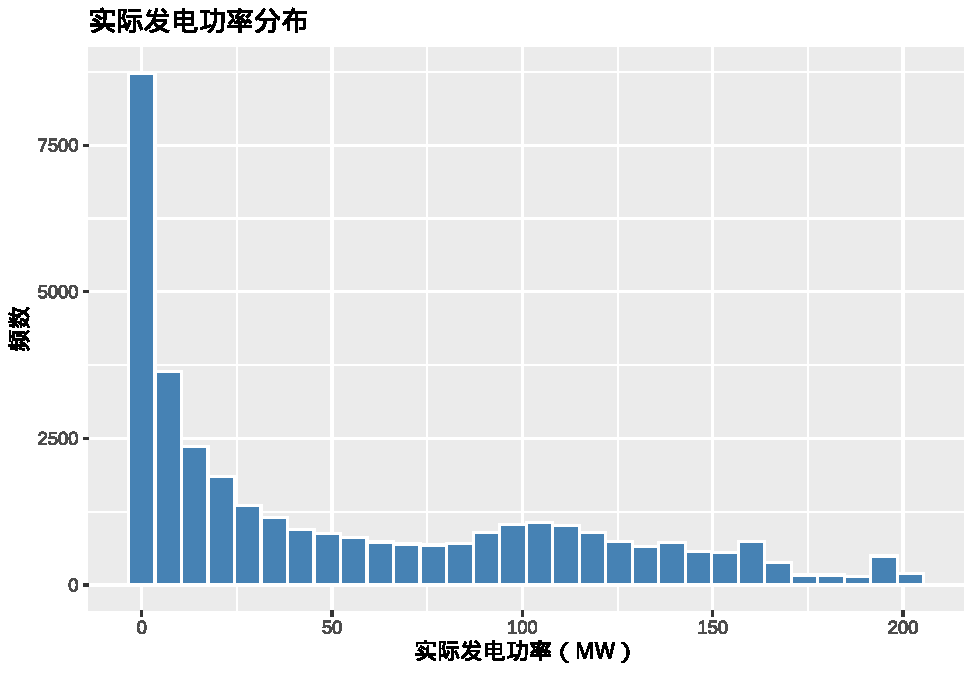
\includegraphics{1_files/figure-latex/unnamed-chunk-2-1.pdf}

\begin{verbatim}
该图展示了实际发电功率的分布情况,横轴为实际发电功率,纵轴为频数。从图中可以看出,发电功率主要集中在低功率范围,此区间的频数明显最高,特别是功率接近0时,频数达到峰值。
随着发电功率的增加,频数迅速下降,中高功率范围的出现频率较低,分布较为均匀。这种分布可能反映了实际运行中低功率状态的设备使用更为频繁,而高功率状态可能仅在需求峰值或特殊情况下出现。

想研究环境对发电的影响,可以从时间、风速、湿度等方面研究
\end{verbatim}

\subsection{按小时可视化发电功率}\label{ux6309ux5c0fux65f6ux53efux89c6ux5316ux53d1ux7535ux529fux7387}

\begin{Shaded}
\begin{Highlighting}[]
\CommentTok{\# geom\_line中设置线段的参数,geom\_point中设置点的参数}
\NormalTok{hourly\_data }\OtherTok{\textless{}{-}}\NormalTok{ data }\SpecialCharTok{\%\textgreater{}\%}
  \FunctionTok{group\_by}\NormalTok{(hour) }\SpecialCharTok{\%\textgreater{}\%}
  \FunctionTok{summarise}\NormalTok{(}\AttributeTok{avg\_power =} \FunctionTok{mean}\NormalTok{(}\StringTok{\textasciigrave{}}\AttributeTok{实际发电功率(mw)}\StringTok{\textasciigrave{}}\NormalTok{, }\AttributeTok{na.rm =} \ConstantTok{TRUE}\NormalTok{))}
\FunctionTok{ggplot}\NormalTok{(hourly\_data, }\FunctionTok{aes}\NormalTok{(}\AttributeTok{x =}\NormalTok{ hour, }\AttributeTok{y =}\NormalTok{ avg\_power)) }\SpecialCharTok{+}
  \FunctionTok{geom\_line}\NormalTok{(}\AttributeTok{color =} \StringTok{"darkorange"}\NormalTok{, }\AttributeTok{size =} \DecValTok{1}\NormalTok{) }\SpecialCharTok{+}
  \FunctionTok{geom\_point}\NormalTok{(}\AttributeTok{color =} \StringTok{"darkblue"}\NormalTok{, }\AttributeTok{size =} \DecValTok{2}\NormalTok{) }\SpecialCharTok{+}
  \FunctionTok{labs}\NormalTok{(}
    \AttributeTok{title =} \StringTok{"一天中不同小时的平均发电功率"}\NormalTok{,}
    \AttributeTok{x =} \StringTok{"小时"}\NormalTok{,}
    \AttributeTok{y =} \StringTok{"平均发电功率(MW)"}
\NormalTok{  )}
\end{Highlighting}
\end{Shaded}

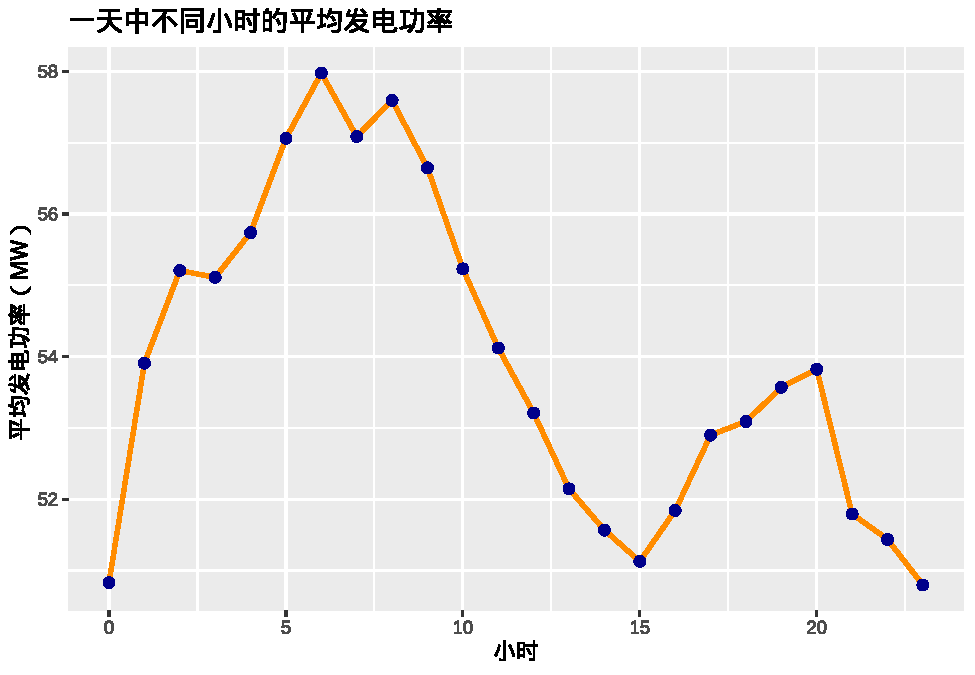
\includegraphics{1_files/figure-latex/unnamed-chunk-3-1.pdf}

\begin{verbatim}
图中展示了一天24小时内发电功率的变化趋势,呈现出典型的日负荷模式。
凌晨至早晨(0-6时)功率逐渐上升,早晨达到高峰;上午至中午(6-12时)功率开始下降;下午继续下降,达到最低点;晚上时段(18-22时)功率回升,并在20时左右达到次高峰;深夜(22-24时)功率迅速下降,进入最低点。     早晚高峰反映了居民和社会活动的规律,午后低谷和深夜低谷则与人们活动减少和设备关闭有关。
\end{verbatim}

\subsection{相关系数矩阵}\label{ux76f8ux5173ux7cfbux6570ux77e9ux9635}

\begin{Shaded}
\begin{Highlighting}[]
\FunctionTok{library}\NormalTok{(reshape2)}
\FunctionTok{library}\NormalTok{(corrplot)}
\CommentTok{\# 计算相关系数矩阵}
\NormalTok{data1 }\OtherTok{\textless{}{-}} \FunctionTok{read\_excel}\NormalTok{(}\StringTok{"./data/新疆风电2019.xlsx"}\NormalTok{)}
\CommentTok{\# 选择数值型列计算相关系数矩阵}
\NormalTok{numerical\_columns }\OtherTok{\textless{}{-}}\NormalTok{ data1[}\FunctionTok{sapply}\NormalTok{(data1, is.numeric)]}

\CommentTok{\# 计算相关系数矩阵}
\NormalTok{cor\_matrix }\OtherTok{\textless{}{-}} \FunctionTok{cor}\NormalTok{(numerical\_columns)}
\CommentTok{\# 使用 corrplot 包绘制相关系数矩阵}
\FunctionTok{corrplot}\NormalTok{(cor\_matrix, }\AttributeTok{method =} \StringTok{"circle"}\NormalTok{, }\AttributeTok{type =} \StringTok{"upper"}\NormalTok{, }\AttributeTok{tl.col =} \StringTok{"black"}\NormalTok{, }\AttributeTok{tl.srt =} \DecValTok{45}\NormalTok{, }\AttributeTok{tl.cex=}\FloatTok{0.6}\NormalTok{)}
\end{Highlighting}
\end{Shaded}

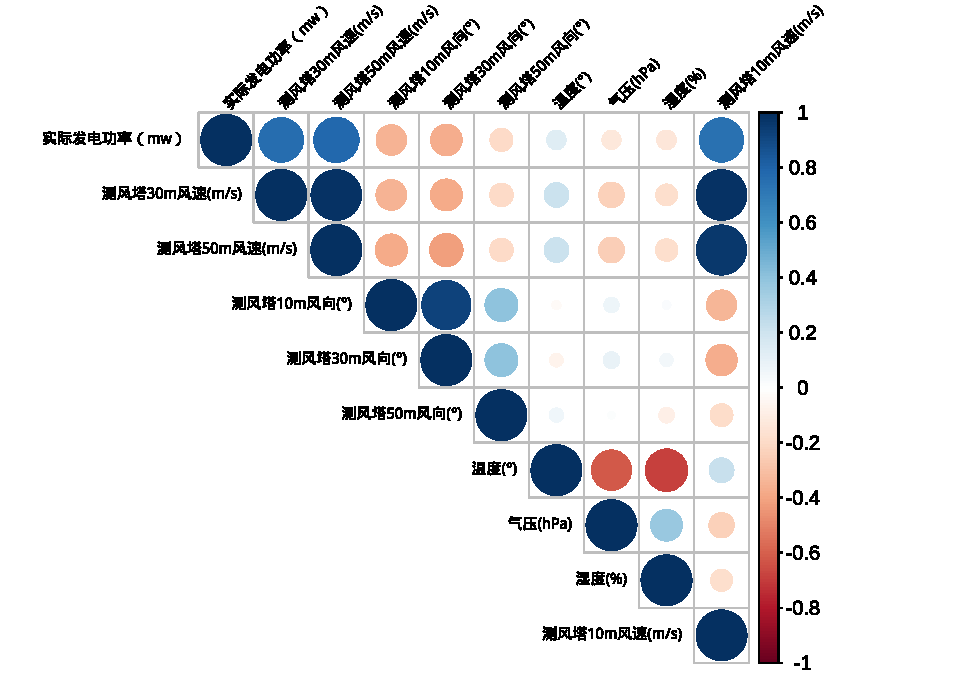
\includegraphics{1_files/figure-latex/unnamed-chunk-4-1.pdf}

\begin{verbatim}
发电功率和风速关系较大,而和其他属性相关性很小,我们可以着重分析发电功率和风速。
\end{verbatim}

\subsection{风速的分布}\label{ux98ceux901fux7684ux5206ux5e03}

\begin{Shaded}
\begin{Highlighting}[]
\CommentTok{\# geom\_density 表示绘制密度图,alpha 表示透明度}
\CommentTok{\# scale\_fill\_brewer 表示用合适的颜色为每个月份的密度图绘制颜色}
\FunctionTok{ggplot}\NormalTok{(data, }\FunctionTok{aes}\NormalTok{(}\AttributeTok{x =} \StringTok{\textasciigrave{}}\AttributeTok{测风塔30m风速(m/s)}\StringTok{\textasciigrave{}}\NormalTok{, }\AttributeTok{fill =}\NormalTok{ month)) }\SpecialCharTok{+}
\FunctionTok{geom\_density}\NormalTok{(}\AttributeTok{alpha =} \FloatTok{0.6}\NormalTok{) }\SpecialCharTok{+}
\FunctionTok{scale\_fill\_brewer}\NormalTok{(}\AttributeTok{palette =} \StringTok{"Set3"}\NormalTok{) }\SpecialCharTok{+}
\FunctionTok{labs}\NormalTok{(}
\AttributeTok{title =} \StringTok{"不同月份 30 米风速分布"}\NormalTok{,}
\AttributeTok{x =} \StringTok{" 风速 (m/s)"}\NormalTok{,}
\AttributeTok{y =} \StringTok{" 密度"}\NormalTok{,}
\AttributeTok{fill =} \StringTok{" 月份"}
\NormalTok{)}
\end{Highlighting}
\end{Shaded}

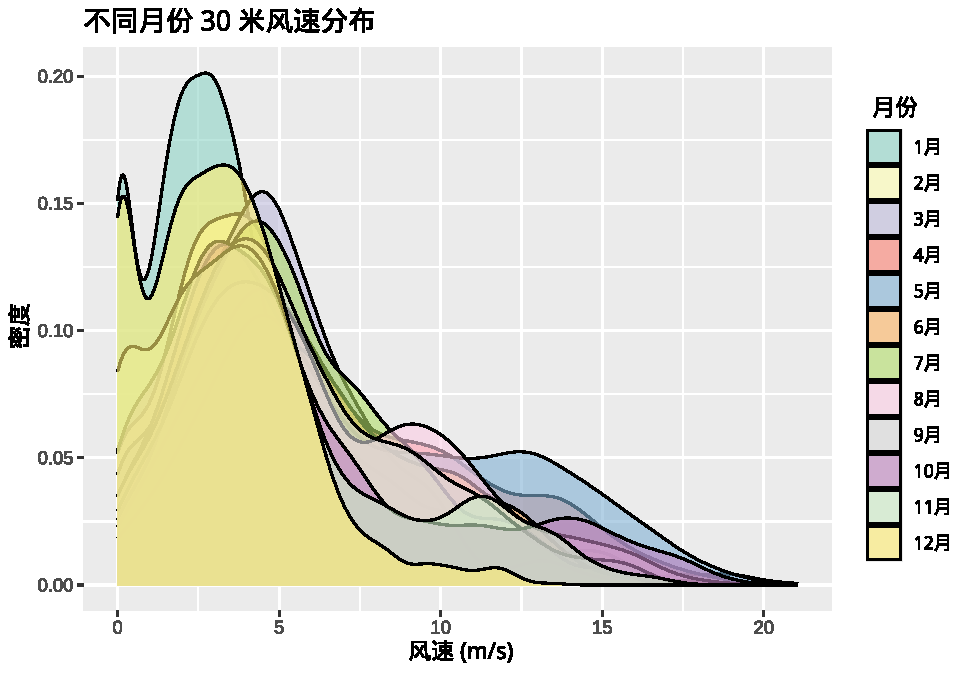
\includegraphics{1_files/figure-latex/unnamed-chunk-5-1.pdf}

\begin{verbatim}
图中展示了不同月份的30米高度风速分布特征,风速大多集中在0\~5 m/s区间,表明低风速发生频率较高,而高风速(\>10 m/s)则较为罕见。
冬季风速分布较窄,集中在低风速区间,反映了天气系统稳定;夏季风速分布较宽,较高风速的概率增大,可能与夏季的对流活动增强有关;春秋季风速分布介于两者之间,表现出过渡特征。
随着季节变化,风速分布逐渐扩展,尤其是高风速的发生概率在春夏季略有增加。
\end{verbatim}

\begin{Shaded}
\begin{Highlighting}[]
\FunctionTok{library}\NormalTok{(reshape2)}
\CommentTok{\# 选择与发电功率和风速相关的列}
\NormalTok{data\_clean }\OtherTok{\textless{}{-}}\NormalTok{ data[, }\FunctionTok{c}\NormalTok{(}\StringTok{"实际发电功率(mw)"}\NormalTok{, }\StringTok{"测风塔30m风速(m/s)"}\NormalTok{, }\StringTok{"测风塔50m风速(m/s)"}\NormalTok{, }\StringTok{"测风塔10m风速(m/s)"}\NormalTok{)]}

\NormalTok{cor\_matrix }\OtherTok{\textless{}{-}} \FunctionTok{cor}\NormalTok{(data\_clean)}
\CommentTok{\# 绘制不同风速与发电功率之间的关系图}
\CommentTok{\# 1. 测风塔30m风速与实际发电功率的关系}
\FunctionTok{ggplot}\NormalTok{(data, }\FunctionTok{aes}\NormalTok{(}\AttributeTok{x =} \StringTok{\textasciigrave{}}\AttributeTok{测风塔30m风速(m/s)}\StringTok{\textasciigrave{}}\NormalTok{, }\AttributeTok{y =} \StringTok{\textasciigrave{}}\AttributeTok{实际发电功率(mw)}\StringTok{\textasciigrave{}}\NormalTok{)) }\SpecialCharTok{+}
  \FunctionTok{geom\_point}\NormalTok{(}\AttributeTok{color =} \StringTok{"blue"}\NormalTok{) }\SpecialCharTok{+}
  \FunctionTok{labs}\NormalTok{(}\AttributeTok{title =} \StringTok{"测风塔30m风速与实际发电功率的关系"}\NormalTok{,}
       \AttributeTok{x =} \StringTok{"测风塔30m风速 (m/s)"}\NormalTok{,}
       \AttributeTok{y =} \StringTok{"实际发电功率 (mw)"}\NormalTok{)}
\end{Highlighting}
\end{Shaded}

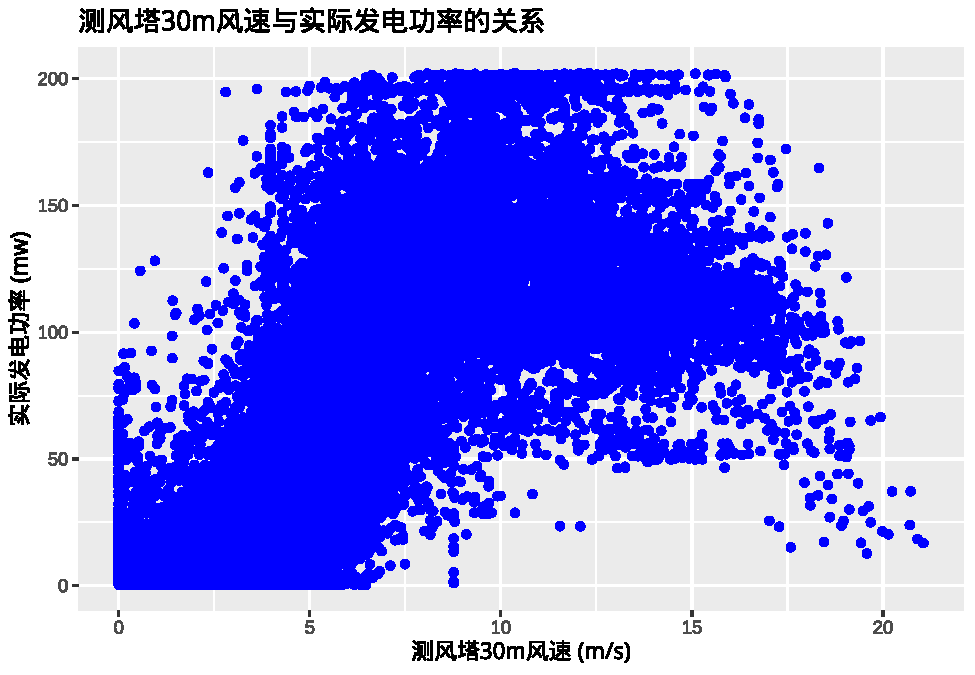
\includegraphics{1_files/figure-latex/unnamed-chunk-6-1.pdf}

\begin{Shaded}
\begin{Highlighting}[]
\CommentTok{\# 2. 测风塔50m风速与实际发电功率的关系}
\FunctionTok{ggplot}\NormalTok{(data, }\FunctionTok{aes}\NormalTok{(}\AttributeTok{x =} \StringTok{\textasciigrave{}}\AttributeTok{测风塔50m风速(m/s)}\StringTok{\textasciigrave{}}\NormalTok{, }\AttributeTok{y =} \StringTok{\textasciigrave{}}\AttributeTok{实际发电功率(mw)}\StringTok{\textasciigrave{}}\NormalTok{)) }\SpecialCharTok{+}
  \FunctionTok{geom\_point}\NormalTok{(}\AttributeTok{color =} \StringTok{"red"}\NormalTok{) }\SpecialCharTok{+}
  \FunctionTok{labs}\NormalTok{(}\AttributeTok{title =} \StringTok{"测风塔50m风速与实际发电功率的关系"}\NormalTok{,}
       \AttributeTok{x =} \StringTok{"测风塔50m风速 (m/s)"}\NormalTok{,}
       \AttributeTok{y =} \StringTok{"实际发电功率 (mw)"}\NormalTok{)}
\end{Highlighting}
\end{Shaded}

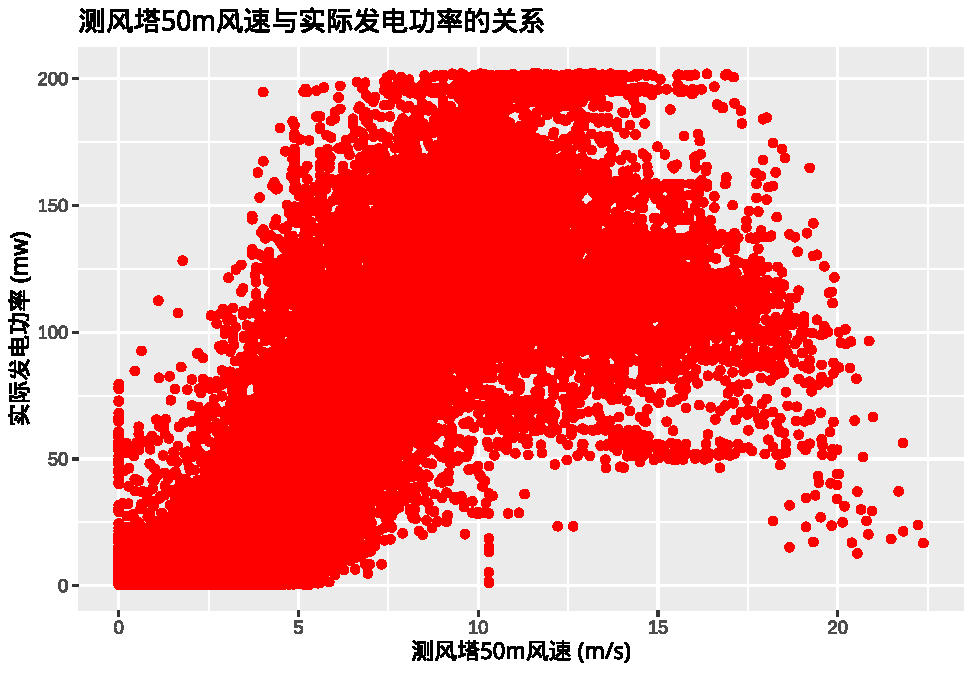
\includegraphics{1_files/figure-latex/unnamed-chunk-6-2.pdf}

\begin{Shaded}
\begin{Highlighting}[]
\CommentTok{\# 3. 测风塔10m风速与实际发电功率的关系}
\FunctionTok{ggplot}\NormalTok{(data, }\FunctionTok{aes}\NormalTok{(}\AttributeTok{x =} \StringTok{\textasciigrave{}}\AttributeTok{测风塔10m风速(m/s)}\StringTok{\textasciigrave{}}\NormalTok{, }\AttributeTok{y =} \StringTok{\textasciigrave{}}\AttributeTok{实际发电功率(mw)}\StringTok{\textasciigrave{}}\NormalTok{)) }\SpecialCharTok{+}
  \FunctionTok{geom\_point}\NormalTok{(}\AttributeTok{color =} \StringTok{"green"}\NormalTok{) }\SpecialCharTok{+}
  \FunctionTok{labs}\NormalTok{(}\AttributeTok{title =} \StringTok{"测风塔10m风速与实际发电功率的关系"}\NormalTok{,}
       \AttributeTok{x =} \StringTok{"测风塔10m风速 (m/s)"}\NormalTok{,}
       \AttributeTok{y =} \StringTok{"实际发电功率 (mw)"}\NormalTok{)}
\end{Highlighting}
\end{Shaded}

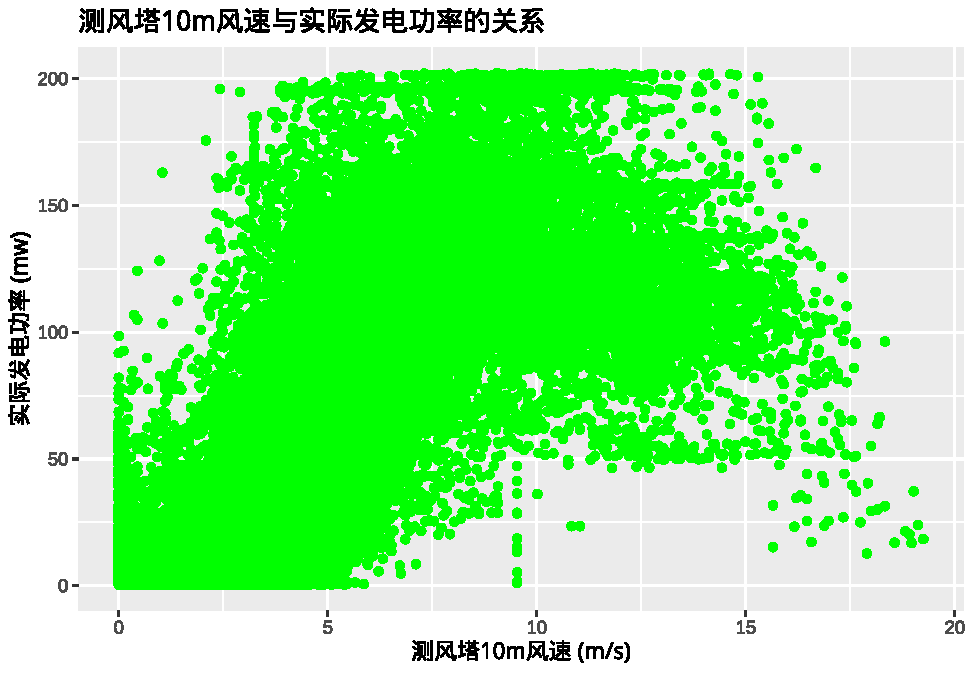
\includegraphics{1_files/figure-latex/unnamed-chunk-6-3.pdf}
这三幅图是不同高度的测风塔,风速与发电功率的关系。

\begin{verbatim}
我们发现并不是风速越快发电功率越高,可能是因为过快的风速会对设备造成损害,或者发电过多造成浪费。
\end{verbatim}

最佳区间在5-10m/s左右。

\subsection{风速与时间和发电功率的关系}\label{ux98ceux901fux4e0eux65f6ux95f4ux548cux53d1ux7535ux529fux7387ux7684ux5173ux7cfb}

\begin{Shaded}
\begin{Highlighting}[]
\CommentTok{\# 绘制双Y轴图}
\FunctionTok{ggplot}\NormalTok{(data, }\FunctionTok{aes}\NormalTok{(}\AttributeTok{x =}\NormalTok{ 时间)) }\SpecialCharTok{+}
  \CommentTok{\# 绘制发电功率曲线,红色}
  \FunctionTok{geom\_line}\NormalTok{(}\FunctionTok{aes}\NormalTok{(}\AttributeTok{y =} \StringTok{\textasciigrave{}}\AttributeTok{实际发电功率(mw)}\StringTok{\textasciigrave{}}\NormalTok{, }\AttributeTok{color =} \StringTok{"发电功率 (MW)"}\NormalTok{), }\AttributeTok{size =} \DecValTok{1}\NormalTok{, }\AttributeTok{alpha =} \FloatTok{0.5}\NormalTok{) }\SpecialCharTok{+}
  \CommentTok{\# 绘制风速曲线,绿色,风速数值乘以10进行缩放,以便与发电功率在同一y轴范围内显示}
  \FunctionTok{geom\_line}\NormalTok{(}\FunctionTok{aes}\NormalTok{(}\AttributeTok{y =} \StringTok{\textasciigrave{}}\AttributeTok{测风塔10m风速(m/s)}\StringTok{\textasciigrave{}} \SpecialCharTok{*} \DecValTok{10}\NormalTok{, }\AttributeTok{color =} \StringTok{"风速 (10m)"}\NormalTok{), }\AttributeTok{size =} \DecValTok{1}\NormalTok{, }\AttributeTok{alpha =} \FloatTok{0.5}\NormalTok{) }\SpecialCharTok{+}
  \CommentTok{\# 设置左侧y轴(发电功率)和右侧y轴(风速)}
  \FunctionTok{scale\_y\_continuous}\NormalTok{(}
    \AttributeTok{name =} \StringTok{"发电功率 (MW)"}\NormalTok{,}
    \AttributeTok{sec.axis =} \FunctionTok{sec\_axis}\NormalTok{(}
      \AttributeTok{trans =} \SpecialCharTok{\textasciitilde{}}\NormalTok{ . }\SpecialCharTok{/} \DecValTok{10}\NormalTok{,  }\CommentTok{\# 将右侧y轴数值恢复到原始风速值}
      \AttributeTok{name =} \StringTok{"风速 (10m) [m/s]"}
\NormalTok{    )}
\NormalTok{  ) }\SpecialCharTok{+}
  \FunctionTok{facet\_wrap}\NormalTok{(}\SpecialCharTok{\textasciitilde{}}\NormalTok{ month, }\AttributeTok{scales =} \StringTok{"free\_x"}\NormalTok{) }\SpecialCharTok{+}
  \FunctionTok{labs}\NormalTok{(}\AttributeTok{x =} \StringTok{"Time"}\NormalTok{, }\AttributeTok{title =} \StringTok{"每月的风速和发电功率关系"}\NormalTok{) }\SpecialCharTok{+}
  \FunctionTok{scale\_color\_manual}\NormalTok{(}\AttributeTok{values =} \FunctionTok{c}\NormalTok{(}\StringTok{"发电功率 (MW)"} \OtherTok{=} \StringTok{"blue"}\NormalTok{, }\StringTok{"风速 (10m)"} \OtherTok{=} \StringTok{"green"}\NormalTok{)) }\SpecialCharTok{+}
  \FunctionTok{theme\_minimal}\NormalTok{() }\SpecialCharTok{+}
  \FunctionTok{theme}\NormalTok{(}
    \AttributeTok{axis.text.x =} \FunctionTok{element\_text}\NormalTok{(}\AttributeTok{angle =} \DecValTok{45}\NormalTok{, }\AttributeTok{hjust =} \DecValTok{1}\NormalTok{),}
    \AttributeTok{axis.text.y =} \FunctionTok{element\_blank}\NormalTok{(),  }\CommentTok{\# 隐藏左侧Y轴的数值}
    \AttributeTok{axis.text.y.right =} \FunctionTok{element\_blank}\NormalTok{(),  }\CommentTok{\# 隐藏右侧Y轴的数值}
    \AttributeTok{legend.title =} \FunctionTok{element\_blank}\NormalTok{(),}
    \AttributeTok{legend.position =} \StringTok{"bottom"}\NormalTok{,  }\CommentTok{\# 将图例放在下面}
    \AttributeTok{legend.box =} \StringTok{"horizontal"}  \CommentTok{\# 图例的布局为横向}
\NormalTok{  )}
\end{Highlighting}
\end{Shaded}

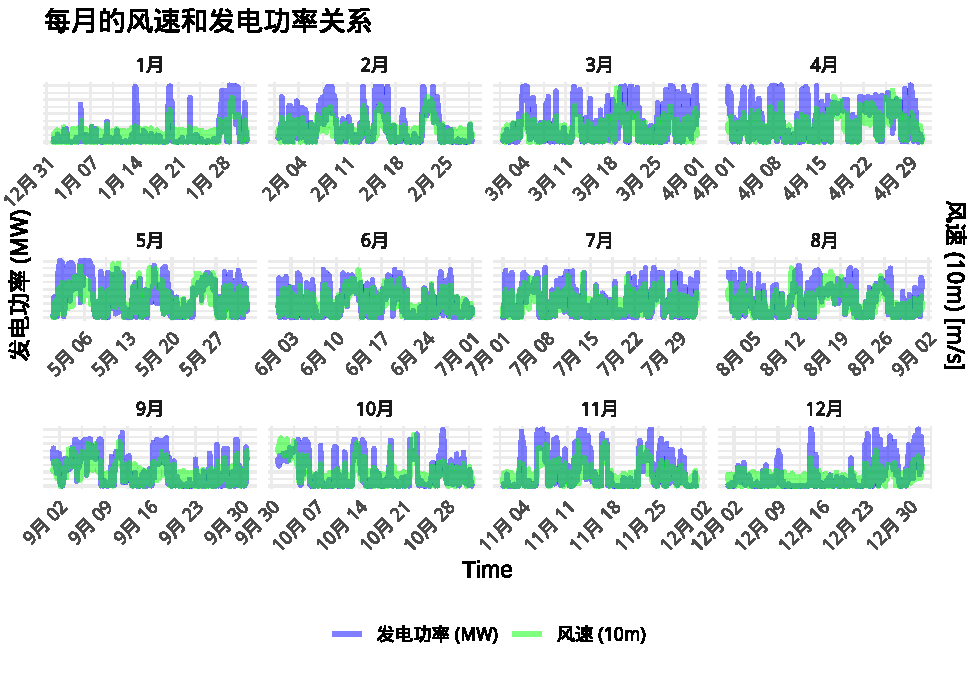
\includegraphics{1_files/figure-latex/unnamed-chunk-7-1.pdf}

\begin{verbatim}
从图中可以看出,风速和发电功率之间存在明显的正相关关系,通常风速较高时,发电功率也较大。

然而,风速与发电功率之间的关系并非完全线性,尤其是在风速变化的极端范围内,发电功率的变化并不会完全按照风速的增加而线性增长,这可能与风力发电系统的功率曲线和效率限制有关。

图中的季节性变化也很明显,某些月份风速较大,导致发电功率随之增加,而其他月份风速较低时,发电功率相应减少。此外,图中还反映了风速和发电功率的波动性,尤其在某些时间点,风速的剧烈波动直接影响了发电功率的波动,这可能由气候变化或设备因素引起。

总体来看,风速和发电功率之间的关系可以帮助优化风力发电系统的效率,同时也揭示了风速变化对系统稳定性的重要影响,尤其是在风速较低或极端变化的情况下,可能需要采取额外的调节措施。
\end{verbatim}

\end{document}
